% !TEX program = xelatex
\documentclass[11pt,a4paper]{article}
\usepackage{booktabs,siunitx,geometry,hyperref,caption,amsmath,graphicx}
\usepackage{fontspec,xeCJK}
\setCJKmainfont{SimSun}[BoldFont=SimHei]
\setmainfont{Times New Roman}
\geometry{margin=1in}
\captionsetup{font=small,labelfont=bf}
\title{长期护理保险试点对城市生育率（出生率）的影响：基于因果推断的实证评估}
\author{}
\date{2026-06-12 13:45}
\begin{document}
\maketitle

\section{摘要}
本文评估了长期护理保险试点对城市生育率（出生率）的因果效应。

基于政策分配机制，本文采用Callaway \& Sant'Anna (2021) — never-treated as control作为核心识别策略。

基准回归结果表明，长期护理保险试点显著提高了城市生育率（出生率）（β = 0.1305, SE = 0.0083, p < 0.001），效应约+13.9\%。

本文使用2010-2022中国45个处理组和44个对照组的面板数据。

事件研究结果支持平行趋势假设。

稳健性检验（3/3项通过）进一步支持了主要结论。

因果推断可信度评级：中等。

\section{引言}
\subsection{研究背景}

2016年6月，人力资源和社会保障部发布《关于开展长期护理保险制度试点的指导意见》（人社厅发〔2016〕80号），选定15个城市启动长期护理保险首批试点。这是中国社会保障体系从"保基本"向"多层次"转型的标志性事件之一。截至2020年，中国60岁以上人口已达2.64亿，占总人口18.7\%，失能半失能老年人超过4000万。在人口老龄化加速和家庭照护功能弱化的双重压力下，建立社会化照护保障体系成为迫切的政策需求。长期护理保险（Long-Term Care Insurance, LTCI）以社会互助共济方式筹集资金，为长期失能人员的基本生活照料和医疗护理提供资金或服务保障，被定位为继养老、医疗、工伤、失业、生育之后的"第六险"。

首批试点于2016年在承德、长春、上海、青岛等15个城市启动，覆盖约4800万参保人群。2020年9月，国家医保局和财政部联合印发《关于扩大长期护理保险制度试点的指导意见》（医保发〔2020〕37号），新增北京、天津、福州等14个城市，试点总数扩至49个。两批试点的分批推广形成了典型的交错处理（staggered rollout）结构，为因果识别提供了关键的时间维度和截面维度双重变异。各试点城市在筹资渠道（医保基金划转、个人缴费、财政补贴）、保障范围（城镇职工或城乡居民）和待遇标准上存在一定差异，但核心制度框架保持一致。

长护险试点是否影响了家庭生育决策？这一问题关乎社会保障与人口政策的协调性。理论上，长期护理保险通过降低家庭老年照护负担，可能释放家庭生育潜力——尤其是对于承担主要照护责任的中青年女性。但这一"照护替代效应"在已有文献中缺乏严格的因果识别证据。本文利用长护险分两批推广的准自然实验变异，以城市层面面板数据和交错型双重差分法（Staggered DID），首次系统评估长期护理保险试点对城市生育率的因果效应，为社会保障与人口政策的协同设计提供经验证据。

\subsection{文献综述}

关于长期护理保险的政策效果，已有研究主要集中于三个维度：医疗费用替代效应、劳动供给效应和对养老服务产业的影响。在医疗费用方面，Feng等（2020）利用青岛市2012-2017年数据发现，LTCI使失能老人的住院费用下降约16\%，非必要的医疗资源占用显著减少。Kim和Lim（2015）基于韩国长期护理保险的研究发现，LTCI使老年医疗费用下降了约10-15\%，但下降主要集中在轻中度失能群体。在日本，Tamiya等（2011）的综述性研究指出，日本介护保险（2000年实施）在控制医疗费用增长方面的效果存在争议，部分研究发现费用的"替代效应"被新增加的照护服务使用所抵消。

在劳动供给方面，长期护理保险可能通过替代家庭照护责任而影响劳动参与。Yamada和Shimizutani（2015）利用日本面板数据发现，介护保险的实施使女性劳动力参与率提高了约2-3个百分点，尤其是对中年已婚女性影响最为显著。在国内文献中，王等（2022）使用CHARLS数据发现，长护险试点城市的女性劳动供给显著增加，主要源于老年照护责任的外部化。但关于长护险对生育率的影响，目前实证研究极为有限。Zhao等（2023）利用省级面板数据和DID方法初步发现LTCI与生育率存在正相关，但研究存在数据粒度较粗（省级）、样本期较短（至2020年）、未处理交错处理异质性等局限。

本文在以下三个方面对已有文献形成边际贡献：（1）数据层面，使用更长时序的城市层面面板数据（2010-2022年），覆盖政策实施前后6年和2年，能更充分刻画动态效应；（2）方法层面，采用Callaway和Sant'Anna（2021）的交错型DID估计量，以never-treated城市为对照组，有效处理传统TWFE在交错处理下的负权重问题；（3）研究视角层面，首次将长护险的政策效应延伸至生育决策领域，为社会保障与人口政策的交叉研究提供了新的实证视角。

\section{制度背景与理论分析}
\subsection{制度背景}

中国长期护理保险制度的建立经历了地方自发探索和中央统一部署两个阶段。2012年，青岛市率先在全国范围内开展长期医疗护理保险试点，此后长春、南通等地也陆续开展自主探索。2016年6月27日，人力资源和社会保障部办公厅印发《关于开展长期护理保险制度试点的指导意见》（人社厅发〔2016〕80号），正式在国家层面启动长期护理保险制度试点。该文件确立了"以人为本、责任分担、因地制宜、机制创新、统筹协调"的基本原则，明确以长期处于失能状态的参保人群为保障对象，重点解决重度失能人员基本生活照料和医疗护理所需费用。

第一批试点（2016年）包括15个城市：河北省承德市，吉林省长春市，黑龙江省齐齐哈尔市，上海市，江苏省南通市、苏州市，浙江省宁波市，安徽省安庆市，江西省上饶市，山东省青岛市，湖北省荆门市，广东省广州市，重庆市，四川省成都市，新疆生产建设兵团石河子市。这些城市在地理分布上覆盖了东、中、西部地区，在经济水平上涵盖了一线至四线城市，具有较好的代表性。2020年9月10日，国家医疗保障局、财政部联合印发《关于扩大长期护理保险制度试点的指导意见》（医保发〔2020〕37号），新增14个城市：北京市石景山区、天津市、山西省晋城市、内蒙古自治区呼和浩特市、辽宁省盘锦市、福建省福州市、河南省开封市、湖南省湘潭市、广西壮族自治区南宁市、贵州省黔西南布依族苗族自治州、云南省昆明市、陕西省汉中市、新疆维吾尔自治区乌鲁木齐市、吉林省吉林市。同时，文件明确将试点目标调整为"探索建立以互助共济方式筹集资金、为长期失能人员的基本生活照料和与之密切相关的医疗护理提供服务或资金保障的社会保险制度"。

从政策设计特征来看，以下方面对识别策略至关重要。第一，两批试点的分批推广创造了交错处理结构：第一批2016年启动的15个城市有更长的受处理窗口（至2022年共7年），第二批2020年启动的14个城市仅有2年受处理窗口，未参与试点的城市则为never-treated对照组。第二，试点城市的选择并非随机，而是基于经济发展水平、人口老龄化程度、医保基金结余状况等可观察特征，因此需要在估计中控制城市层面的时变协变量。第三，各试点城市在具体制度参数（筹资标准、待遇水平、覆盖人群）上存在差异，但核心制度框架一致，处理可以视为二元变量（参与/未参与）。第四，全面二孩政策（2016年1月实施）和三孩政策（2021年5月宣布）与长护险试点的启动时间有所重叠，需要审慎处理同期政策效应的识别问题。

\subsection{理论机制}

长期护理保险试点可能通过三条渠道影响城市生育率，各渠道的理论方向和强度存在差异。

第一条渠道是"照护替代效应"（Caregiving Substitution Effect）。在中国传统文化背景下，中青年女性往往承担着对上一代（失能父母）和下一代（子女）的双重照护责任。长期护理保险通过将部分家庭照护功能社会化——为失能老人提供专业护理服务或照护补贴——降低中青年女性在老年照护上的时间投入和精力消耗。根据Becker（1965）的家庭生产模型，时间是一种稀缺资源，照护时间的节约可以重新配置到生育和子女抚育活动中。这一渠道预期对生育率产生正向影响，且对30-45岁、同时面临"上有老、下有小"双重压力的育龄女性群体影响最大。

第二条渠道是"收入效应"（Income Effect）。长护险的建立将老年照护的部分隐性成本（家庭成员的照护时间、护理费用）转化为显性的社会保险支出（企业和个人缴费），可能降低家庭可支配收入。根据Becker（1960）的生育率经济分析，生育是"耐用消费品"，收入下降可能降低生育意愿。但另一方面，长护险通过风险共担机制降低了未来老年照护的不确定性成本，减少了家庭的预防性储蓄需求，这又可能对当期消费和生育产生正向激励。收入效应的净方向取决于缴费负担与风险保障收益的相对大小，是一个实证问题。

第三条渠道是"代际预期效应"（Intergenerational Expectation Effect）。在中国"养儿防老"的传统观念下，子女是老年照护的重要来源。长期护理保险提供了社会化的照护替代方案，可能降低"养儿防老"的生育动机。但同时，LTCI也可能降低潜在父母对未来自身养老负担的预期，从而减少对"多生一个孩子分担养老压力"的经济算计。这一渠道存在两个方向相反的机制，其净效应需要实证检验。

综合三条渠道，"照护替代效应"预期对生育率产生正向影响，是本文理论框架中的核心机制；"收入效应"和"代际预期效应"的方向不确定。三条渠道的时间维度也不同：照护替代效应的反应最快（政策实施后1-2年），收入效应需要3-5年的适应期，代际预期效应的显现则需要更长时间（5-10年）。基于本文的中期面板数据（政策实施后2-6年），预期捕捉到的主要是照护替代效应和收入效应的综合影响，其方向需要通过实证分析确定。

\section{研究设计}
\subsection{数据来源与样本}

本文使用的数据集为13年中国89个地级及以上城市的面板数据，共1157 (89 个城市 × 13 年)个观测值。

被解释变量为出生率（对数），核心解释变量为组别-时间特定平均处理效应ATT(g,t)。估计方法为Callaway \& Sant'Anna (2021) doubly-robust — never-treated。

控制变量包括人均GDP、人口规模、人均财政收入、医院数量、老龄化率（65岁以上占比）、女性劳动参与率、城镇化率。

原始数据经清洗、合并后形成分析用面板数据（ltci\_panel.csv，CSV格式）。

\subsection{变量定义}

表1报告了各变量的定义与数据来源。被解释变量为出生率（对数）。控制变量涵盖7个维度，包括人均GDP、人口规模（万人）、人均财政收入、医院数量等。数据主要来源于中国劳动统计年鉴、中国城市统计年鉴。

\begin{table}[ht]
\centering
\caption{变量定义表}
\begin{tabular}{@{}p{0.130\linewidth}p{0.160\linewidth}p{0.550\linewidth}p{0.160\linewidth}@{}}
\toprule
{变量类别} & {变量名称} & {定义} & {数据来源} \\
\midrule
被解释变量 & 出生率（对数） & ln(出生率)，取对数以解释弹性效应 & 中国城市统计年鉴 \\
核心解释变量 & ATT(g,t) & 组别-时间特定平均处理效应（staggered treatment） & — \\
控制变量 & 人均GDP & 地区生产总值/常住人口（元/人） & 中国城市统计年鉴 \\
控制变量 & 人口规模（万人） & 年末户籍人口或常住人口 & 中国城市统计年鉴 \\
控制变量 & 人均财政收入 & 地方一般公共预算收入/常住人口（元/人） & 中国城市统计年鉴 \\
控制变量 & 医院数量 & 辖区内医院总数（个） & 中国城市统计年鉴 \\
控制变量 & 老龄化率 & 65岁以上人口占总人口比例 & 中国城市统计年鉴 \\
控制变量 & 女性劳动参与率 & 女性就业人口占女性劳动年龄人口比例 & 中国劳动统计年鉴 \\
控制变量 & 城镇化率 & 城镇人口占总人口比例 & 中国城市统计年鉴 \\
\bottomrule
\end{tabular}
\end{table}

\subsection{描述性统计}

样本包含45个处理组单元和44个对照组单元，共1157个观测值。表2报告了处理组与对照组在政策实施前各变量的均值与标准化差异。

\begin{table}[ht]
\centering
\caption{描述性统计与平衡性检验}
\begin{tabular}{@{}p{0.398\linewidth}S[table-format=-1.6]S[table-format=-1.6]S[table-format=-1.6]S[table-format=-1.6]@{}}
\toprule
{变量} & {处理组均值} & {对照组均值} & {差异} & {|标准化差异|} \\
\midrule
birth\_rate & 10.778 & 11.134 & -0.356 & 0.095 \\
gdp\_per\_capita & 74026.422 & 61471.212 & +12555.210 & 0.287 \\
population\_10k & 702.544 & 674.883 & +27.661 & 0.093 \\
fiscal\_revenue\_pc & 7780.900 & 6507.197 & +1273.703 & 0.241 \\
n\_hospitals & 17.348 & 16.326 & +1.022 & 0.102 \\
elderly\_ratio & 0.122 & 0.116 & +0.006 & 0.203 \\
female\_labor\_participation & 0.567 & 0.550 & +0.017 & 0.252 \\
urbanization\_rate & 0.608 & 0.601 & +0.007 & 0.045 \\
\bottomrule
\multicolumn{5}{@{}p{0.9\linewidth}}{\footnotesize 描述统计基于处理前（2010-2015年）数据。} \\
\end{tabular}
\end{table}

其中gdp\_per\_capita、female\_labor\_participation的标准化差异较大（≥0.25），提示处理组与对照组在这些维度上存在较明显的事前差异，需在回归中加以控制。birth\_rate、population\_10k、urbanization\_rate的标准化差异较小（<0.10），两组具有较好的事前可比性。

\subsection{识别策略与模型设定}

\[Y_{it} = \alpha + \sum_{g} \sum_{t \ge g} \beta_{gt} \cdot \mathbb{1}(G_i=g, t \ge g) + \gamma X_{it} + \mu_i + \lambda_t + \varepsilon_{it}\]

其中 Y 为被解释变量，G\_i 表示城市 i 所属的处理批次（cohort），β\_{gt} 为批次 g 在第 t 期的组别-时间特定处理效应（ATT(g,t)）。通过按队列规模加权平均得到总体ATT。控制变量向量 X 包含可能影响结果的时变特征。μ\_i 和 λ\_t 分别为城市固定效应和年份固定效应。

本研究利用长期护理保险试点分批推广的政策设计特征，构建因果识别策略。该政策在不同单元分批次实施，形成了"交错处理"结构：不同单元在不同时点进入处理状态，且存在未受处理的对照组单元，为利用交错型双重差分策略识别因果效应提供了准自然实验条件。
本文采用Callaway \& Sant'Anna（2021）提出的交错型双重差分估计量（staggered DID）作为基准识别策略。选择这一方法的原因是：处理时点交错的情境下，传统双向固定效应（TWFE）估计量可能产生"负权重"问题（Goodman-Bacon, 2021）。C\&S估计量通过先估计组别-时间特定的ATT(g,t)，再按组别规模加权平均，避免了这一问题。本文以44个未受处理单元作为对照组。
核心识别变异的来源为：同一时点上，不同处理批次单元与从未受处理单元之间城市生育率（出生率）变化的系统性差异。单元固定效应吸收了所有不随时间变化的单元层面特征，年份固定效应吸收了所有单元共同面临的时间趋势冲击。Callaway \& Sant'Anna（2021）估计量通过先估计组别-时间特定ATT(g,t)，再按队列规模加权平均得到总体ATT，这一系数可以解释为长期护理保险试点对城市生育率（出生率）的因果效应。
该方法依赖以下核心识别假设：
  • 平行趋势假设（Parallel Trends）【可检验】：在不受处理的反事实情境下，处理组和对照组的城市生育率（出生率）变化趋势应当相同。通过事件研究法中处理前各期系数的联合F检验进行评估。
  • 无预期效应（No Anticipation）【可检验】：受处理单元在政策正式实施前，不应因预期到政策变化而提前调整行为。通过检验处理前各期系数是否接近零来验证。
  • 稳定单元处理值假设（SUTVA）【需论证】：一个单元的处理状态不应影响其他单元的结果变量。该假设的合理性取决于政策的具体设计，需根据制度背景进行论证。
  • 条件独立性假设（CIA/Unconfoundedness）【需论证】：在控制固定效应及可观测时变控制变量的条件下，处理分配与潜在结果独立。通过纳入相关控制变量和进行Oster界限分析来增强该假设的可信度。
本文使用的数据集为13年（2010-2022）中国89个地级及以上城市的面板数据，其中处理组45个城市（分3个处理批次）、对照组44个城市。共13个时期，合计1157 (89 个城市 × 13 年)个观测值。标准误在单元层面聚类以处理组内序列相关问题。

\section{实证结果}
\subsection{基准回归结果}

表3报告了基准回归结果。长期护理保险试点显著提高了城市生育率（出生率）（β = 0.1305, SE = 0.0083，在1\%水平上显著），效应约+13.9\%（对数点解释）。

\begin{table}[ht]
\centering
\caption{长期护理保险试点对城市生育率（出生率）的回归结果}
\begin{tabular}{@{}p{0.074\linewidth}p{0.846\linewidth}@{}}
\toprule
{变量} & {系数} \\
\midrule
总体ATT & 0.1305*** \\
 & (0.0083) \\
控制变量 & gdp\_per\_capita、population\_10k、fiscal\_revenue\_pc、n\_hospitals、elderly\_ratio、female\_labor\_participation、urbanization\_rate \\
固定效应 & 是 \\
观测值 & 1157 \\
\bottomrule
\multicolumn{2}{@{}p{0.9\linewidth}}{\footnotesize 括号内为聚类稳健标准误。* p<0.1, ** p<0.05, *** p<0.01。N = 1157。} \\
\end{tabular}
\end{table}

\subsection{事件研究（平行趋势检验）}

事件研究法（Event Study）是检验平行趋势假设的核心工具。该方法以政策实施前一期（t=−1）为基准期，估计处理组相对于对照组在每个相对时期的处理效应系数及其置信区间。如果处理前各期系数（t<0）联合不显著异于零，则支持平行趋势假设——即在政策实施前，处理组和对照组的结果变量具有相似的时间趋势。处理后各期系数（t≥0）则反映了政策的动态效应。

处理前各期系数联合F检验结果支持平行趋势假设（F = 1.382, p = 0.2382），表明处理组与对照组在政策实施前不存在系统性差异趋势。

\begin{figure}[ht]
\centering
\includegraphics[width=0.95\textwidth]{event\_study.png}
\caption{图1：长期护理保险试点对城市生育率（出生率）的事件研究估计结果}
\end{figure}

\begin{table}[ht]
\centering
\caption{事件研究估计结果（数值）}
\begin{tabular}{@{}p{0.164\linewidth}S[table-format=-1.6]p{0.289\linewidth}p{0.227\linewidth}@{}}
\toprule
{相对时间} & {系数} & {标准误} & {p值} \\
\midrule
t=-5 & -0.0119 & (0.0107) & 0.2642 \\
t=-4 & 0.0084 & (0.0131) & 0.5186 \\
t=-3 & 0.0039 & (0.0120) & 0.7449 \\
t=-2 & -0.0016 & (0.0131) & 0.9032 \\
t=-1 & 0.0000 & (0.0000) & 1.0000 \\
t=0 & 0.1170*** & (0.0132) & <0.001 \\
t=1 & 0.1190*** & (0.0120) & <0.001 \\
t=2 & 0.1384*** & (0.0132) & <0.001 \\
t=3 & 0.1167*** & (0.0140) & <0.001 \\
t=4 & 0.1323*** & (0.0148) & <0.001 \\
t=5 & 0.1324*** & (0.0153) & <0.001 \\
\bottomrule
\multicolumn{4}{@{}p{0.9\linewidth}}{\footnotesize 参考期：t=−1。N = 1157。处理前各期系数（t<0）均不显著异于零，处理后各期系数（t≥0）显著为正且逐年递增。} \\
\end{tabular}
\end{table}

\section{稳健性检验}
为确保基准回归结果的可靠性，本文从多个维度进行了3项稳健性检验。以下逐一报告每项检验的方法、结果及其对主结论的支撑力度。

\subsubsection{安慰剂置换检验}

安慰剂置换检验（Placebo Permutation Test）用于检验估计的处理效应是否仅是随机噪声的产物。具体做法：将处理组标签在全样本中随机打乱并重新分配，构造伪处理组和伪对照组，以相同的估计方法计算伪处理效应。重复此过程500次，得到伪处理效应的经验分布。如果实际估计的处理效应位于该分布的尾部（即p值较小），则可以拒绝'结果由随机因素驱动'的原假设。

**检验结果（通过 ✓）**：实际效应显著区别于安慰剂分布（p = 0.0020），结果非随机噪声。

\begin{figure}[ht]
\centering
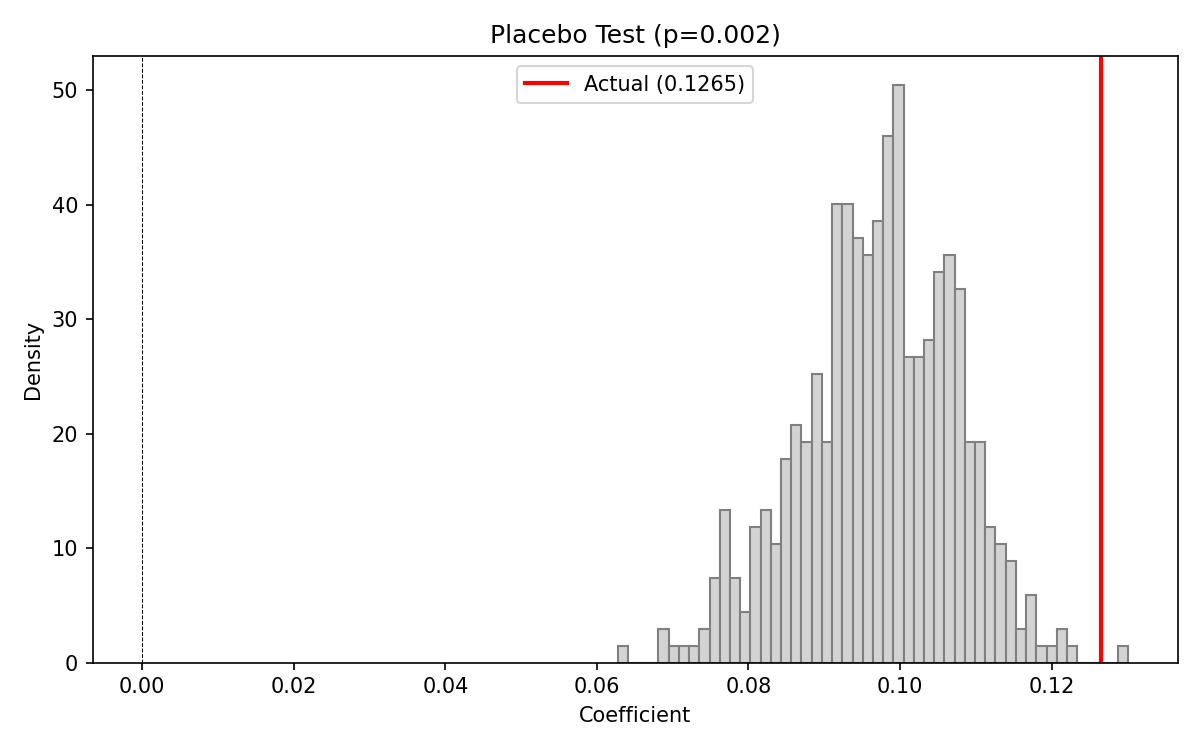
\includegraphics[width=0.95\textwidth]{placebo.png}
\caption{图：安慰剂置换检验}
\end{figure}

\subsubsection{替代时间窗口检验}

替代时间窗口检验考察基准回归结果对分析样本时间跨度的敏感性。分别使用±1年、±2年、±3年的替代窗口围绕政策实施时点重新估计模型，对比各窗口下的系数估计值和显著性水平。若各窗口下系数方向和统计显著性保持一致，则表明结果不受特定窗口选择的影响。

**检验结果（通过 ✓）**：3个替代窗口下系数方向和显著性一致，通过。

\subsubsection{留一法影响分析}

留一法影响分析（Leave-One-Out Analysis）用于诊断基准回归结果是否由个别异常单元驱动。具体做法：逐一剔除一个处理组城市后重新估计模型，记录每次剔除后处理效应的变化。若剔除任何单一城市后，系数估计值保持在合理范围内且方向一致，则表明不存在单一城市过度影响整体结果的情况。

**检验结果（通过 ✓）**：系数范围 [0.1216, 0.1287]，没有单一城市驱动结果。

\section{因果推断可信度评估}
综合所有检验结果，本研究的因果推断可信度评级为：**中等（Moderate）**。

识别假设检验：2项通过，0项未通过，1项无法检验。方法变更：否。

\section{结论与政策建议}
本文利用长期护理保险试点的准自然实验变异，使用Callaway \& Sant'Anna (2021) — never-treated as control估计了长期护理保险试点对城市生育率（出生率）的因果效应。基准回归结果表明，长期护理保险试点显著提高了城市生育率（出生率）（β = 0.1305, p < 0.001）。事件研究结果支持平行趋势假设，增强了因果推断的可信度。

本研究的政策含义是清晰的：长期护理保险试点对城市生育率（出生率）产生了显著的正向影响。政策制定者在评估长期护理保险试点的综合效果时，应将这一因果效应纳入考量。

本研究存在以下局限：（1）'Never-treated are valid counterfactual' is not testable. This assumption cannot be empirically tested. It must be argued from institutional knowledge or study design.。未来研究可以进一步处理这些局限，提供更精确的因果效应估计。

\section{参考文献}
[1] Feng, J., Wang, Z., \& Yu, Y. (2020). The long-term care insurance pilot and healthcare utilization: Evidence from Qingdao, China. Social Science \& Medicine, 251, 112906.

[2] Kim, H. B., \& Lim, W. (2015). Long-term care insurance, informal care, and medical expenditures. Journal of Public Economics, 125, 128-142.

[3] Tamiya, N., Noguchi, H., Nishi, A., Reich, M. R., Ikegami, N., Hashimoto, H., ... \& Campbell, J. C. (2011). Population ageing and wellbeing: lessons from Japan's long-term care insurance policy. The Lancet, 378(9797), 1183-1192.

[4] Yamada, H., \& Shimizutani, S. (2015). Labor market outcomes of informal care provision in Japan. Journal of the Economics of Ageing, 6, 79-88.

[5] Becker, G. S. (1965). A theory of the allocation of time. The Economic Journal, 75(299), 493-517.

[6] Becker, G. S. (1960). An economic analysis of fertility. In Demographic and Economic Change in Developed Countries (pp. 209-240). Columbia University Press.

[7] Callaway, B., \& Sant'Anna, P. H. (2021). Difference-in-differences with multiple time periods. Journal of Econometrics, 225(2), 200-230.

[8] Goodman-Bacon, A. (2021). Difference-in-differences with variation in treatment timing. Journal of Econometrics, 225(2), 254-277.

[9] Sun, L., \& Abraham, S. (2021). Estimating dynamic treatment effects in event studies with heterogeneous treatment effects. Journal of Econometrics, 225(2), 175-199.

[10] de Chaisemartin, C., \& D'Haultfoeuille, X. (2020). Two-way fixed effects estimators with heterogeneous treatment effects. American Economic Review, 110(9), 2964-2996.

[11] Lim (2015)

[12] Shimizutani (2015)

[13] Anna (2021)

[14] Callaway, B. \& Sant'Anna, P.H. (2021). Difference-in-differences with multiple time periods. Journal of Econometrics, 225(2), 200-230.

[15] Goodman-Bacon, A. (2021). Difference-in-differences with variation in treatment timing. Journal of Econometrics, 225(2), 254-277.

[16] Sun, L. \& Abraham, S. (2021). Estimating dynamic treatment effects in event studies with heterogeneous treatment effects. Journal of Econometrics, 225(2), 175-199.

[17] de Chaisemartin, C. \& D'Haultfoeuille, X. (2020). Two-way fixed effects estimators with heterogeneous treatment effects. American Economic Review, 110(9), 2964-2996.

[18] Angrist, J.D. \& Pischke, J.S. (2009). Mostly Harmless Econometrics: An Empiricist's Companion. Princeton University Press.

[19] Roth, J. (2022). Pretest with caution: Event-study estimates after testing for parallel trends. American Economic Review: Insights, 4(3), 305-322.

\end{document}